\documentclass[UTF8,10.5pt,a4paper]{ctexart}
\usepackage[margin=1.7cm,headheight=15pt]{geometry}
\usepackage{amsmath,amssymb,booktabs,graphicx,xcolor,fancyhdr,hyperref,enumitem}
\hypersetup{colorlinks=true,linkcolor=blue,urlcolor=blue,pdftitle={漂移扩散方程数值实验临时报告},pdfauthor={}}
\definecolor{deepblue}{HTML}{0D2659}
\ctexset{section={format=\Large\bfseries\color{deepblue}},subsection={format=\normalsize\bfseries}}
\setlength{\parindent}{2em}\setlength{\parskip}{.35em}
\setlist{nosep,leftmargin=2em}\setlength{\tabcolsep}{6pt}
\pagestyle{fancy}\fancyhf{}\fancyhead[L]{漂移扩散方程数值实验}\fancyhead[R]{临时报告 · 2026-11-17}\fancyfoot[C]{\thepage}
\newcommand{\fig}[2]{\begin{center}\includegraphics[width=#2\linewidth]{figures/#1.pdf}\end{center}}
\begin{document}
\begin{center}{\LARGE\bfseries 漂移扩散方程的数值实验}\\[.5em]
{\large 反向随机游走与 Gaussian 宽核直接卷积}\\[.5em]
Rcpp、RcppArmadillo 与 C++ OpenMP 并行计算
\end{center}
\noindent\textbf{摘要}\quad
在同一零 Dirichlet 边界问题上，实现逐步吸收的反向随机游走和经过指数变换、奇延拓的 Gaussian 直接卷积。完成 23 项串行 E0 测试及另行 7 项 OpenMP 集成核验；正式实验采用两线程，并以一、二、四线程比较性能。R 层串行组织实验与参考计算；C++ 求解器采用 OpenMP 并行。随机游走同时报告抽样误差与离散偏差，卷积分别考察核截断和网格求积误差。本文的性能及精度结论均来自本轮 OpenMP 原始记录。

\section{问题、基准与实验环境}
研究
\[
u_t=a u_x+D u_{xx},\quad 0<x<1;\qquad
u(0,t)=u(1,t)=0,\quad u(x,0)=f(x).
\]
固定 $a=0.2,D=0.05,T=0.5$，令 $\beta=a/(2D)=2$、$\gamma=a^2/(4D)=0.2$。主初值和解析解为
\[
f(x)=e^{-2x}\sin(\pi x),\qquad
u_\star(x,t)=e^{-2x-(0.05\pi^2+0.2)t}\sin(\pi x).
\]
该解满足初边值条件及 PDE，可独立核验求解器。网格有 $N$ 段、$N+1$ 个节点，$h=1/N$。内部 RMSE 与最大误差单独计算，边界不混入内部指标。主基准只衰减振幅，不用于说明一般信号的峰移动。
\begin{center}\small
\begin{tabular}{ll}\toprule
项目 & 本轮设置\\\midrule
硬件 & Intel Core i7-11800H，8 物理核 / 16 逻辑核，31.74 GiB RAM\\
系统 & Windows 11 x64（build 26200）\\
计算软件 & R 4.6.1，Rcpp 1.1.2，RcppArmadillo 15.6.0-1\\
编译与数值库 & GCC 14.3.0（Rtools45），Armadillo 15.6.0，默认 BLAS\\
并行 & C++ OpenMP，正式精度实验 $p=2$，性能 $p=1,2,4$ 线程\\
随机性 & L'Ecuyer-CMRG，主种子 20261116，完整任务状态已保存\\
精度与重复 & 双精度，MC 每配置 30 批，性能预热后 7 次\\\bottomrule
\end{tabular}
\end{center}
正式 E1--E6 从已有编译缓存执行共约 \textbf{44.7 秒}，包含预热、批量测量、首次线程请求核验和实验阶段写出，不包含首次编译、绘图与文稿编译。R 层不创建工作进程；BLAS 设为单线程，避免嵌套并行。该耗时仅代表本机本次运行。
\newpage
\section{方法一：反向随机游走与正确性}
时间离散为 $n$ 步、$\tau=T/n$，令
\[
r=D\tau/h^2,\quad b=a\tau/(2h),\quad
p_-=r-b,\quad p_0=1-2r,\quad p_+=r+b.
\]
检查三个概率非负且和为 1。路径从查询节点出发，以 $p_-,p_0,p_+$ 左移、停留、右移；每一步检查端点，触边立即吸收，收益记零。存活到最后才取终点初值：
\[
Y=f(X_n)\mathbf1_{\{\text{未触边}\}},\qquad
\widehat u=\frac1M\sum_{k=1}^M Y_k.
\]
被吸收路径仍占分母。$+a u_x$ 下后向路径偏向右，是读取初值的方向。C++ 一次接收全部逻辑路径块，用 OpenMP 分配块；每块独立 RNG 状态，线程内部不调用 R API。
\subsection{区分抽样与离散误差}
小规模参照为内部转移矩阵 $Q$，下、主、上对角依次为 $p_-,p_0,p_+$；端点概率流失，不归一化边缘行。计算
\[
U_{\rm disc}=Q^nf_{\rm int},\qquad
v=Q^n(f_{\rm int}^2)-(Q^nf_{\rm int})^2,
\]
则 $\mathbb E(\widehat u-u_\star)^2=(U_{\rm disc}-u_\star)^2+v/M$。
每块返回贡献和、平方和、路径数、存活数和实际步数。样本方差用分母 $M-1$，标准误为 $\widehat s_Y/\sqrt M$。30 批 RMSE 先对平方误差取平均再开方，未用 30 批平均后的误差冒充单次预算精度。
\subsection{串行小规模测试}
23 项 E0 测试全部通过，日志见 \texttt{results/tests/e0\_tests.csv}。小规模测试固定一线程。
\begin{center}\small
\begin{tabular}{p{.27\linewidth}p{.61\linewidth}}\toprule
测试 & 核验内容与结果\\\midrule
已知一步期望 & $N=4,\tau=0.1$，初值 $[0,1,0,0,0]$，内部期望 $[0.84,0.04,0]$\\
强制路径 & 首次左右触边收益 0、步数 1；停留路径步数正确\\
R 与 Rcpp 随机流 & 同状态产生相同统计，误差低于 $10^{-12}$\\
MC 统计检查 & 10 批 $M=4096$ 总均值在离散期望的约四个标准误内\\
宽核与边界 & 手算宽核、奇延拓、有限核正弦恒等式及原始边界残差通过\\
输入与退化情形 & 零初值、$T=0$、非法概率、越界索引及非零边界处理通过\\\bottomrule
\end{tabular}
\end{center}
R 参考路径用于正确性核验，正式计算用 Rcpp；矩阵参照与解析计算在性能计时之外。该矩阵参考不是本项目的卷积算法。另完成 7 项专门 OpenMP 集成核验，包括实际线程数、串并行位级一致性、CMRG 与 R 路径及输入只读检查，与本组串行 E0 分开记录。
\newpage
\section{随机游走实验：路径数与网格}
E1 采用 $(N,n)=(8,8),(16,32)$，$x=1/8$，均有 $r=0.2$，各扫描四档 $M$、独立 30 批，正式按 16 个逻辑块并行。E2 复用共同配置，仅新增 $(32,128),M=4096$。
\fig{mc_error}{1}
\begin{center}\small
\begin{tabular}{rrrrr}\toprule
$N$ & $M$ & 对离散期望 RMSE & 对解析解 RMSE & 30 批标准差\\\midrule
8 & 256 & $1.17\times10^{-2}$ & $1.15\times10^{-2}$ & $1.17\times10^{-2}$ \\
8 & 4096 & $3.15\times10^{-3}$ & $3.77\times10^{-3}$ & $3.19\times10^{-3}$ \\
8 & 16384 & $1.20\times10^{-3}$ & $2.67\times10^{-3}$ & $1.22\times10^{-3}$ \\
16 & 256 & $1.29\times10^{-2}$ & $1.28\times10^{-2}$ & $1.28\times10^{-2}$ \\
16 & 4096 & $2.75\times10^{-3}$ & $2.71\times10^{-3}$ & $2.75\times10^{-3}$ \\
16 & 16384 & $1.83\times10^{-3}$ & $1.94\times10^{-3}$ & $1.86\times10^{-3}$ \\
\bottomrule\end{tabular}
\end{center}
粗网格 $N=8$ 的离散偏差为 $2.39\times10^{-3}$，$M=16384$ 时总 RMSE 为 $2.67\times10^{-3}$。细网格偏差较小，但有限 30 批的估计会波动，不能要求每一档都精确符合理论斜率。
\fig{mc_grid}{.88}
$N=8,16,32$ 的离散偏差分别约 $2.39\times10^{-3}$、$5.75\times10^{-4}$、$1.42\times10^{-4}$；固定 $M=4096$ 的总 RMSE 同时受抽样噪声影响，噪声可以遮住网格改善。
\newpage
\section{方法二：正确边界的 Gaussian 直接卷积}
先消去漂移：
\[
v=e^{\beta x+\gamma t}u,\qquad g=e^{\beta x}f,\qquad v_t=Dv_{xx}.
\]
对 $g$ 作关于两个端点的奇延拓，形成周期 2 的 $\widetilde g$，则
\[
u(x,T)=e^{-\beta x-\gamma T}
\int_{\mathbb R}\frac{e^{-z^2/(4DT)}}{\sqrt{4\pi DT}}\widetilde g(x-z)\,dz.
\]
奇延拓与对称热核使两端贡献成对抵消。这里的周期性属于辅助填充，物理边界仍为零；直接对原始初值补零、普通镜像或周期化不能替代这一步。

对整数索引 $m$，令 $q=((m\bmod 2N)+2N)\bmod2N$，
\[
g_{\rm ext}(m)=
\begin{cases}g_q,&0\le q\le N,\\-g_{2N-q},&N<q<2N.\end{cases}
\]
该规则处理负下标和超过一个区间的窗口。核权重与一次终态求和为
\[
w_\ell=\frac{h}{\sqrt{4\pi DT}}e^{-(\ell h)^2/(4DT)},\qquad
U_j=e^{-\beta x_j-\gamma T}\sum_{\ell=-K}^K w_\ell g_{\rm ext}(j-\ell).
\]
这是一维图像滤波式宽窗口内积，不使用三点核、FFT 或时间推进。权重含 $h$，截断后不再归一化。有限窗口近似完整边界积分表示，其误差须实测。
\subsection{为什么采用这个核长度}
Gaussian 核的方差为 $2DT$，标准差 $s_T=\sqrt{2DT}$。覆盖 $c$ 个标准差对应
\[
K=\left\lceil c s_T/h\right\rceil,\qquad W=2K+1.
\]
向上取整保证物理半径至少为 $c s_T$；奇数长度包含中心和左右各 $K$ 点，保留对称抵消。$c=1,2,3,4,6$ 的连续双尾质量约为 $0.3173,0.04550,0.002700,6.33\times10^{-5},1.97\times10^{-9}$。它们只提示截断规模，未包含离散求积误差。
\subsection{实现与并行}
\begin{enumerate}
\item RcppArmadillo 准备变换初值、完整奇延拓、Gaussian 权重和指数因子。
\item 每点用 \texttt{arma::dot(padded.subvec(...),weights)}，输入只读、输出独立。
\item C++ 用 \texttt{omp parallel for schedule(static)} 按独立输出点并行，线程共享完整只读填充输入，不在分界处重新补零。
\item 记录端点置零前残差，再将输出端点置为精确零。
\end{enumerate}
全场成本 $O(NW)$，共享工作数组 $O(N+K)$；只查询 $q$ 点时求和成本 $O(qW)$。主实验最大置零前边界残差为 $2.50\times10^{-17}$。
\newpage
\section{卷积实验：核大小与网格求积}
E3 固定 $N=512$，仅改变覆盖倍数；以同网格 $c=8$ 结果诊断截断，另用 $c=10$ 检查参考。两参考之差的内部 RMSE 为 $3.82\times10^{-16}$。
\fig{kernel}{1}
\begin{center}\small
\begin{tabular}{rrrrr}\toprule
$c$ & $W$ & 内部 RMSE & 求解中位/ms & 预热后新输入/ms\\\midrule
1 & 231 & $3.84\times10^{-2}$ & 0.109 & 0.343 \\
2 & 459 & $1.12\times10^{-3}$ & 0.160 & 0.435 \\
3 & 689 & $4.65\times10^{-4}$ & 0.218 & 0.444 \\
4 & 917 & $1.62\times10^{-5}$ & 0.295 & 0.550 \\
6 & 1375 & $1.90\times10^{-10}$ & 0.404 & 0.722 \\
\bottomrule\end{tabular}
\end{center}
从 $c=1$ 到 $c=4$，RMSE 从 $3.84\times10^{-2}$ 降至 $1.62\times10^{-5}$；$c=6$ 达到 $1.90\times10^{-10}$。加宽核增加内积工作；完整时间还包含本地准备、R/C++ 调用和 OpenMP fork/join，短调用可能有测量波动。

E4 固定物理覆盖 $c=8$，随网格更新 $K$。使用 $f_{\rm poly}=e^{-2x}x(1-x)$，避免单一正弦初值过早达到舍入平台。其参照为
\[
u_{\rm poly}=e^{-2x-0.2T}
\sum_{k\ {\rm odd}}\frac{8}{\pi^3k^3}e^{-D(k\pi)^2T}\sin(k\pi x).
\]
最高奇数波数 31 与 63 的参照在本次节点上差异低于 $10^{-12}$。
\par\noindent
\begin{minipage}{.60\linewidth}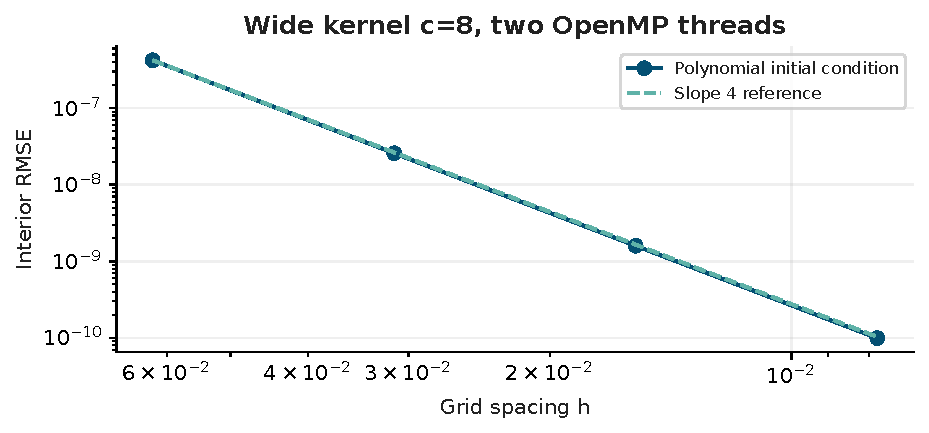
\includegraphics[width=\linewidth]{figures/grid.pdf}\end{minipage}
\begin{minipage}{.38\linewidth}\centering\small
\begin{tabular}{rrr}\toprule
$N$ & RMSE & 观测阶\\\midrule
16 & $4.22\times10^{-7}$ & -- \\
32 & $2.58\times10^{-8}$ & 4.033 \\
64 & $1.59\times10^{-9}$ & 4.014 \\
128 & $9.92\times10^{-11}$ & 4.006 \\
\bottomrule\end{tabular}
\end{minipage}

本输入的观测阶为 4.01--4.03，属于该输入及设置下的结果，不能推广为任意初值的统一收敛阶。E3 与 E4 分开控制核半径和网格。
\newpage
\section{串行、并行与计算开销}
R 层仅串行组织实验，两个 C++ 求解器用 OpenMP 并行循环。MC 每点固定 16 个逻辑路径块，L'Ecuyer-CMRG 状态绑定逻辑块；线程各自更新私有 RNG，完成后按块编号固定顺序归约。卷积按独立输出点并行，输入共享只读，每窗口保持原顺序求和。改变线程数不改变样本或求和顺序，串并行预测和 MC 计数核对一致。每个性能配置预热后计时 7 次，短任务批量测量，线程数顺序按轮次交错。
\fig{parallel_time}{1}
\begin{center}\small
\begin{tabular}{lrrrrr}\toprule
任务 & $p$ & 中位/ms & [Q1,Q3]/ms & 加速比 & 效率\\\midrule
MC & 1 & 183.70 & [181.69, 184.76] & 1.00 & 100.0\% \\
MC & 2 & 95.45 & [93.71, 95.79] & 1.92 & 96.2\% \\
MC & 4 & 52.70 & [51.53, 55.33] & 3.49 & 87.2\% \\
卷积 & 1 & 110.37 & [109.44, 112.70] & 1.00 & 100.0\% \\
卷积 & 2 & 56.97 & [56.25, 57.61] & 1.94 & 96.9\% \\
卷积 & 4 & 30.20 & [29.67, 30.87] & 3.66 & 91.4\% \\
\bottomrule\end{tabular}
\end{center}
上表 MC 取 $N=64,n=256,M=65536$；卷积取 $N=8192,c=4,W=14657$。本次四线程中位时间之比为 \textbf{3.49} 和 \textbf{3.66}，效率为 87.2\% 和 91.4\%。个别 $S_p$ 略高于 $p$ 可由有限次数计时、频率及调度波动引起，不构成超线性加速保证。
\fig{speedup}{.87}
$N=512$ 卷积单线程 0.427 ms、四线程 0.213 ms。$t_{\rm solve}$ 含 R/C++ 调用、fork/join、调用内准备、计算、包装与归约；$t_{\rm prepare\_call}=0$，无 IPC。首次请求两、四线程并核验的 R 包装调用分别观测 1.001 ms、0.534 ms，含检查且可能复用 libgomp 既有线程。$t_{\rm once}$ 是该单次观测加 $t_{\rm input}+t_{\rm solve}$，不是新 R 进程端到端冷启动或纯 C++ 核心耗时。随机流分配、编译、独立预热、真值与绘图在计时外。
\newpage
\section{共同任务、结论与复现}
E6 固定主问题和共同 8 点 $x=(1,3,\ldots,15)/16$、两线程。MC 使用 $N=16,n=32$，每点 $M$ 条路径、每配置 30 批；卷积使用 $N=512$，仅计算共同 8 个窗口，每配置计时 7 次。
\fig{cost}{.92}
\begin{center}\small
\begin{tabular}{lrrr}\toprule
配置 & 共同点 RMSE & 预热后新输入/ms & 加首次请求观测/ms\\\midrule
Gaussian, $c=2$ & $1.12\times10^{-3}$ & 0.279 & 1.3 \\
Gaussian, $c=3$ & $4.64\times10^{-4}$ & 0.290 & 1.3 \\
Gaussian, $c=4$ & $1.62\times10^{-5}$ & 0.288 & 1.3 \\
MC, $M=1024$ & $4.45\times10^{-3}$ & 2.189 & 3.2 \\
MC, $M=4096$ & $2.44\times10^{-3}$ & 5.606 & 6.6 \\
MC, $M=16384$ & $1.12\times10^{-3}$ & 19.425 & 20.4 \\
\bottomrule\end{tabular}
\end{center}
MC 的 $M=16384$ 与卷积的 $c=2$ 观测 RMSE 分别为 $1.12\times10^{-3}$、$1.12\times10^{-3}$，预热后的新输入成本为 19.425 ms、0.279 ms，相差约 \textbf{69.6 倍}。加本次首次请求核验观测后为 20.426 ms、1.280 ms，成本比为 16.0。该结论仅针对本次一维、常系数、齐次边界任务。

\textbf{结论与局限。} 增加路径数降低 MC 抽样误差，细网格降低离散偏差；直接卷积在本任务更易达到高精度，宽核成本与核长相关。OpenMP 收益依赖规模、线程开销和硬件。有限 30 批不保证逐次误差达标。本轮只覆盖两种方法，未验证一般变系数、非零边界和高维，亦未进行正式课程提交。

\textbf{复现。} 先按 README 编译并运行串行 E0 与 OpenMP 集成测试，再在根目录运行：
\begin{flushleft}\small\ttfamily
Rscript scripts/02\_run.R --mode full --experiment all --threads 2 --run-id NEW\\
python scripts/03\_summarise\_plot.py NEW
\end{flushleft}
\noindent\texttt{results/openmp-final-20261117/} 保留配置、完整 RNG 状态、539 条原始计时和源文件哈希。首次安装编译另需时间。

{\footnotesize
\textbf{资料与 AI 使用。} 数学与实验口径见 \texttt{numeric-experiment-plan.md}，并行方式依照 \texttt{idea.md} 及课程 OpenMP 讲义。AI 辅助方案、实现、统计与文稿，通过串行参考、解析真值、23 项串行 E0 及另 7 项 OpenMP 集成核验。所有图表来自本轮原始记录。
\begin{enumerate}[leftmargin=1.5em]
\item RcppArmadillo：\url{https://github.com/RcppCore/RcppArmadillo}
\item R parallel：\url{https://stat.ethz.ch/R-manual/R-devel/library/parallel/html/RngStream.html}
\item 课程仓库：\texttt{computer-skill/openmp-basics.md}，Rcpp 与 OpenMP、图像卷积练习。
\item 反射法：Masayuki Yano, ESC384 Lecture Notes, Lecture 7，2021。
\item 演示主题：用户提供的 CleanEasy BeamerTheme，Jose Paulo Marchezi，保留模板许可。
\end{enumerate}}
\end{document}
